% !TeX spellcheck = en_US
\section{Overall system architecture and services}
\label{sec:concept:sysarchitecture}
\todo{highlight the differences between optimal (proposed) infrastructure and the implementation}
\todo{We vs. I}

Based on the accomplishments of current model repositories (\emph{BioModels database} and \emph{PMR2}), we want to reach further and not only design a concept to simply store multiple versions of a model, but to enrich the version hops with additional information -- more specifically we decided to store deltas between versions, to allow for more specific search queries or analysis of changes between versions.
As base system \masymos was chosen, since it already provides good import methods for both model formats this work focuses on (\sbml and \cellml) and uses \neoj as underlaying database system (cf. Section \ref{sec:background:graph-db:masymos}). The graph-based approach of \neoj allows to store highly interlinked heterogeneous data in a efficient, easily querieable way -- making it the perfect match for \sysbio models and deltas of them (cf. Section \ref{sec:background:graph-db:neo4j}).  

Since \masymos was build as an index database for models, it is not possible to reconstruct a \xml model document out of \masymos itself. Consequently all files need to be made accessible in another way. For this purpose I choose a static HTTP server, which serves all model files, organized in a specific folder structure. The structure is is described in detail in Section \ref{sec:concept:filestorage}.
Said structure is generated by the \modelcrawler, when gathering all model versions from a variety of repositories. As Figure \ref{fig:system-overview} indicates, the \modelcrawler (cf. Section \ref{sec:impl:masymos}) crawls the model files and stores them in the file system, accessible via a HTTP server. Following it sends an request, to the \rest API of \masymos, called \morre, which in turn pulls the model from the HTTP server and inserts it into \neoj, using subroutines of the \masymos implementation.

The \modelcrawler in fact is a product of my former activity at the department of \sysbio and Bioinformatics at the University of Rostock, hence it is not directly part of this work. However it is essential for the prototype implementation and therefore describe in Section \ref{sec:impl:modelcrawler}.

Once all desired model versions are imported into \masymos via the \morre interface, the  asynchronous diff generation can be triggered, using a \rest endpoint from the to be implemented diff \rest interface. Alternatively the generation can be activated periodically by a cron job or by a database trigger, in case a new model version is inserted.
However, triggering a generic diff-generation-job, will first start a gathering task in the \masymos-diff plugin, which searches for direct version hops without a diff and submits accordingly a diff generation task for each version hop. 
Later task will then fetch the \xml documents of both versions from the HTTP server and interface \bives to compare those versions. The result is consequently analyzed and translated into a graph structure (cf. Section \ref{sec:concept:dbmodel}) and inserted into the database.

As shown in Figure \ref{fig:system-overview}, the main part of the implementation splits into two projects: the diff \rest plugin and the \masymos-diff plugin. This separation is intended to mimic the project structure of \masymos itself, which was meant to separate public APIs from the actual implementation, so it is easy to build multiple front ends, for instance a Command Line Interface (CLI) for easier debugging during development phases. Consequently I followed this example as well and also used a CLI during development.
\todo{actually add the CLI to the figure}

\begin{figure}[h]
	\centering
	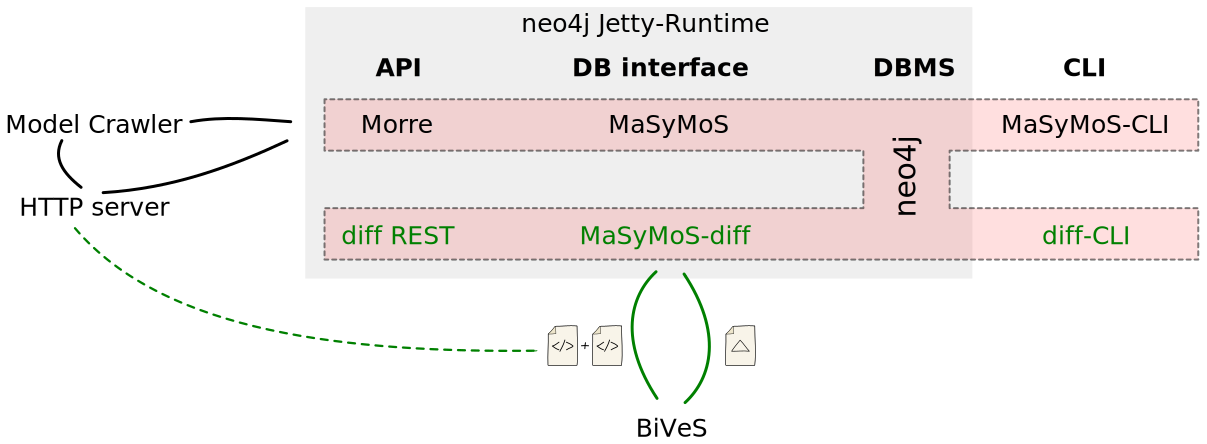
\includegraphics[width=\textwidth]{resources/system-overview-matrix.pdf}
	\caption{Infrastructure overview}
	\begin{flushleft}
		Shown is the intended system architecture of \masymos \neoj and additional services. New implementations are displayed in green, whereby the parts directly extending \neoj are situated in a red box.
	\end{flushleft}
	\label{fig:system-overview}
\end{figure}

\section{Database model and storage decisions}
\label{sec:concept:dbmodel}
\begin{comment}
\begin{itemize}
\item extension to database model cf. \ref{fig:db-model}
	\subitem linking version
	\subitem storing differences
\item decisions on storage model
	\subitem storing each version full (no delta-storage)
	\subitem each version is aware to the search index
	\subitem diff still enables for analysis of changes
	\subitem higher storage consumption
\item extended storage model
\end{itemize}
\end{comment}
% description of ER model
Figure \ref{fig:db-er-model} shows the proposed database schema as ER model. To reduce complexity and redundancy, the storage structure of models in \masymos is simplified, shown on the left hand side of the figure. Further the \comodi ontology (cf. Section \ref{sec:background:onto:comodi}) is not remodeled, but instead represented as generic \texttt{OntologyTerm}.

\todo{Add color to the diagram, to ease explanation}
\todo{Find out, to what a Diff can link}

The schema is organized around a \texttt{Diff} entity linking two \texttt{Document} entities, which represent an (XML-)document containing a model. The interlink is expressed via the \texttt{has\_diff} relation, which can be expressed in two roles: \texttt{source} and \texttt{destination}. I decided to use these terms in order to prevent confusion regarding the time line of the model versions, since \bives also does not discriminate any temporal information.
This 2-hop relation does not necessarily need to span between two consecutive versions, but I decided for a standard setup it might be less useful to store differences between every possible combination of versions, since it would consume unreasonable amount of storage. Further are deltas concatable, so it does not take any significant computational effort to generate a diff for larger version steps out of consecutive diffs.

Every \texttt{Diff} entity links to one or multiple \texttt{DiffEntry} via the \texttt{has\_entry} relation.  
A \texttt{DiffEntry} can be either a \texttt{DiffInsert},  \texttt{DiffDelete}, \texttt{DiffMove} or a \texttt{DiffUpdate} entity, following the terms used by \bives \cite{Scharm2015} and \comodi \cite{Scharm2016}.

Each \texttt{DiffEntry} represents a difference detected by \bives \cite{Scharm2015} and links to at least on \texttt{ModelEntity} via either \texttt{is\_source}, a \texttt{is\_destination}, or both, depending on the type of the difference.
For instance a \texttt{DiffInsert} links to a \texttt{ModelEntity} of the \emph{destination} with a \texttt{is\_destination} relation.
In contrast a \texttt{DiffDelete} links to the \emph{source} version with \texttt{is\_source} to a \texttt{ModelEntity}. Whereby \texttt{DiffMove} and \texttt{DiffModify} use both relations \texttt{is\_source} - linking to the \emph{source} - and \texttt{is\_destination} - linking to the \emph{destination} version.

Additionally a \texttt{DiffEntry} can link to an \texttt{OntologyTerm}, which again are hierarchical structured, but not modeled in this ER model. Those terms are currently only taken from the \comodi ontology \cite{Scharm2016}, cf. Section \ref{sec:background:onto:comodi}, since no other ontology exists, describing changes.

\todo{add table (or similar) of all entities and relations in the appendix}
\todo{make visible, that ER model is just a sub-ER}

This storage structure, I decided on, does not make use of efficient reverse-delta storage, as traditional VCS (cf. Section \ref{sec:background:manage-versions:traditional-vcs}), instead each model is stored complete for multiple reasons: It allows for a very lose coupling to the base \masymos implement ion, means the diff-extension is additive to the features of \masymos and does not require for intrusive changes of the code base. Further the core functionality of \masymos, providing a full text and structural search index, is not disturbed, so if required each version of a model can be treated as single instance. Resulting in easier structural analyses per model version and less expensive operations on the indexes, when inserting a new model version.

On the other hand the complete storage of each model increases the database size significantly. But to keep the scope of this work concise and the implementation reasonable, I focused on a good data interlinkage and less on a storage efficient data model. \todo{revise?}
\todo{Add argument, that \masymos is only search index and does not allow for model reconstruction from the database}
\todo{mention, what is stored in attributes}

\begin{figure}
	\centering
	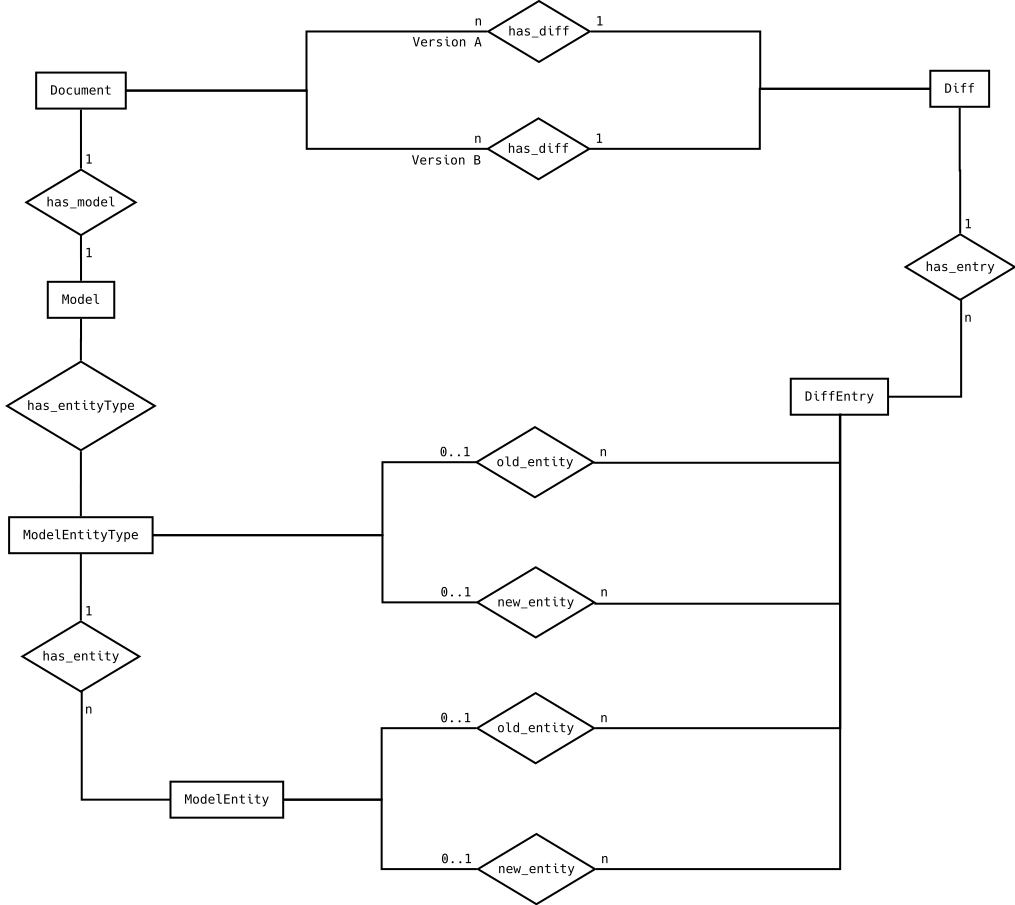
\includegraphics[width=\textwidth]{resources/db-concept-er.pdf}
	\caption{ER model of the proposed database schema}
	\label{fig:db-er-model}
\end{figure}

\begin{figure}[h]
	\includegraphics[width=\textwidth]{resources/db_structure.jpg}
	\caption{Proposed database structure}
	\label{fig:db-model}
\end{figure}

\section{The HTTP file server}
\label{sec:concept:filestorage}
